%% Complete Article for JIKI Journal
%% Based on Fauzan Husain's research on thermodynamic properties of magnetic models
%% Using Monte Carlo simulations with vertex-cubic spin model

\documentclass[conference, compsoc, twoside]{IEEEtran}

% Essential packages
\usepackage[numbers,sort&compress]{natbib}
\usepackage[labelsep=period,labelfont=bf,justification=justified,font=small]{caption}
\usepackage{balance}
\usepackage{graphicx}
\usepackage{amsmath}
\usepackage{array}
\usepackage[english]{babel}
\usepackage{blindtext}
\usepackage{url}
\usepackage{listings}
\usepackage{inconsolata}
\usepackage[bottom]{footmisc}
\usepackage[top=3cm,bottom=3cm,left=3cm,right=3cm]{geometry}
\usepackage{fancyhdr}
\usepackage{hyperref}

% Code listing setup
\lstset{
  basicstyle=\ttfamily,
}
\captionsetup[lstlisting]{font={small}, labelfont={bf}}

% Header setup
\setlength{\headheight}{22pt}
\pagestyle{fancy}
\fancyhf{}
\setcounter{page}{1}
\fancypagestyle{firststyle}
{
   \fancyhf{}
   \chead{Jurnal Ilmu Komputer dan Informasi (Journal of Computer Science and Information) \\ 15/1 (2022), xx-xx. DOI: \url{http://dx.doi.org/xx/jiki.v15xx.xxx}}
   \fancyfoot[C]{\thepage}
}

\renewcommand{\headrulewidth}{0pt}
\fancyhead[LE]{\thepage \textbf{\space \textit{Jurnal Ilmu Komputer dan Informasi (Journal of Computer Science and Information),}} \textit{volume 15,} \\ \textit{ \textrm{ } issue 1, February 2022}}
\fancyhead[LO]{\textit{Fauzan Husain et.al., Thermodynamic Properties of Magnetic Models}}
\fancyhead[RO]{\thepage}

% URL line breaks
\renewcommand{\UrlBreaks}{\do\-}

% Figure and table setup
\def\figurename{Fig.}%
\def\tablename{Table}%

% Path to pictures
\graphicspath{{../pics/}}

\begin{document}

\title{Thermodynamic Properties of Magnetic Models Using Monte Carlo Simulations: A Study of Vertex-Cubic Spin Systems}

\author{\IEEEauthorblockN{Fauzan Husain, Tasrief Surungan\\\\}
	\IEEEauthorblockA{
		\normalfont Department of Physics, Faculty of Mathematics and Natural Sciences, Hasanuddin University, Makassar, Indonesia\\\\
		\textit{Email: fauzanhusain17@gmail.com, tasrief@gmail.com} 
	} \\
}

\twocolumn[
{\csname @twocolumnfalse\endcsname \maketitle}
{\csname @twocolumnfalse\endcsname 
	\renewcommand{\abstractname}{Abstract}
	\begin{abstract}
		\noindent
		\normalfont 
		This research investigates the thermodynamic properties of magnetic models using Monte Carlo simulations with vertex-cubic spin systems. The study focuses on analyzing phase transitions, magnetization behavior, and critical temperature estimation in layered lattice structures. Using the Wolff algorithm for spin updates, we simulate systems with varying lattice sizes (8×8 to 32×32) and layer configurations (1-3 layers). Results show that increasing lattice size sharpens phase transition characteristics, while additional layers shift critical temperatures to higher values and enhance magnetic order stability. The vertex-cubic spin model effectively captures collective behavior in quasi-three-dimensional systems, providing insights into magnetic material properties and phase transition phenomena.
		\\\\
		\noindent
		\textbf{Keywords}: \textit{magnetic models, Monte Carlo simulation, phase transitions, vertex-cubic spin, thermodynamic properties} \\\\
	\end{abstract}
	
	\renewcommand{\abstractname}{Abstrak}
	\begin{abstract}
		\noindent
		\normalfont 
		Penelitian ini menyelidiki sifat-sifat termodinamika model magnetik menggunakan simulasi Monte Carlo dengan sistem spin vertex-kubik. Studi ini berfokus pada analisis transisi fasa, perilaku magnetisasi, dan estimasi suhu kritis dalam struktur kisi berlapis. Menggunakan algoritma Wolff untuk pembaruan spin, kami mensimulasikan sistem dengan ukuran kisi bervariasi (8×8 hingga 32×32) dan konfigurasi lapisan (1-3 lapisan). Hasil menunjukkan bahwa peningkatan ukuran kisi mempertegas karakteristik transisi fasa, sementara penambahan lapisan menggeser suhu kritis ke nilai yang lebih tinggi dan meningkatkan stabilitas orde magnetik. Model spin vertex-kubik secara efektif menangkap perilaku kolektif dalam sistem kuasi-tiga dimensi, memberikan wawasan tentang sifat material magnetik dan fenomena transisi fasa.
		\\\\
		\noindent
		\textbf{Kata Kunci}: \textit{model magnetik, simulasi Monte Carlo, transisi fasa, spin vertex-kubik, sifat termodinamika} \\\\
	\end{abstract}
}
]

\IEEEpeerreviewmaketitle
\thispagestyle{firststyle}

\section{Introduction}

Thermodynamics developed rapidly in the mid-19th century through contributions from figures such as Carnot, Joule, Clausius, and Kelvin, who built the theoretical framework for explaining the macroscopic behavior of physical systems. Meanwhile, kinetic gas theory and the concept of entropy developed by Boltzmann connected molecular dynamics with entropy, forming the foundation for the birth of statistical mechanics. This discipline not only explains macroscopic order but also spontaneous fluctuations that occur naturally in physical systems \cite{Pathria2001}.

Research on the thermodynamic properties of magnetic materials has been central to condensed matter physics for several decades, not only because of the richness of physical phenomena it offers but also because of its potential applications in technology, from data storage to computational materials. Understanding how microscopic spin interactions (magnetic moments) influence macroscopic system behavior when exposed to temperature or magnetic field changes is the primary goal of this study. The classification of magnetic materials based on their response to external magnetic fields is illustrated in Fig.~\ref{fig:magnetic_classification}.

Phase transitions represent one of the most fascinating aspects of statistical physics, where changes in macroscopic parameters such as temperature or pressure can trigger drastic changes in the collective structure and properties of a system, for example from paramagnetic phase (no magnetic order) to ferromagnetic (long-range magnetic order) in magnetic materials or vice versa. Studies of phase transitions not only reveal fundamental material properties but also provide insights into the universality of system behavior near critical points, regardless of microscopic details \cite{Tokura2019}. Fig.~\ref{fig:magnetic_phase_transition} shows the typical behavior of magnetic phase transitions.

In general, phase transitions are related to the phenomenon of system symmetry breaking. For phase changes caused by thermal fluctuations, the system is at a high degree at high temperatures because all configuration spaces are allowed. Decreasing temperature will reduce thermal fluctuations and result in properties being in a stable state \cite{Surungan2017}.

One important phenomenon in phase changes is the occurrence of spontaneous magnetization. In ferromagnetic systems, when the temperature is lowered until reaching a certain temperature called the critical temperature, spontaneous magnetization will occur. The system undergoes a phase change from a paramagnetic system to a ferromagnetic system. The critical temperature $T_c$ for ferromagnetic systems is called the Curie temperature. This phenomenon is very interesting to study because it involves spin interactions, which are microscopic factors.

Ernest Ising (1925) introduced a model that can explain the spontaneous magnetization phenomenon of ferromagnetic (FM) systems. The Ising model is a simple form of the Heisenberg model to solve the model proposed by Lenz (1920) in studying FM phase changes at Curie temperature. This model contains discrete variables representing the magnetic moment of atomic spins with values $s = \pm 1$. These spins are modeled in a lattice where each spin can interact with its nearest neighbors. Fig.~\ref{fig:ising_model} illustrates the spin orientations in the Ising model.

The 2D Ising model is one example of a simple statistical model to show spontaneous magnetization in a system. In this study, we will examine the cubic spin model, which is one of the discrete spin models with polyhedral symmetry. Polyhedral symmetry for spin models is obtained by dividing the 4$\pi$ solid angle equally from the sphere structure. There are five possible types of models from polyhedral structures: tetrahedron, octahedron, hexahedron, icosahedron, and dodecahedron, as shown in Fig.~\ref{fig:platonic_solids}.

These spins are modeled in a lattice that interacts with each other like the Ising model. Using the Monte Carlo simulation method, the order parameter can be calculated and the critical temperature of each model can be estimated. For this research, it is specifically focused on studying the vertex-cubic spin model, with vertices numbered as illustrated in Fig.~\ref{fig:cube_vertices}.

In previous research \cite{Surungan2008}, FM systems on 2D lattices were studied, and other research \cite{Sutiono2013} studied systems with different lattice structures, namely layered lattices (3D). Systems with larger spatial dimensions are theoretically expected to have higher critical temperatures because the number of neighbors from each spin is greater. Fig.~\ref{fig:layered_lattice} shows an illustration of the layered square lattices used in our simulations.

This research specifically focuses on studying the thermodynamic properties of magnetic models with vertex-cubic spin models arranged on lattices of size $L \times L \times n$. Spin interactions are defined through scalar products of spin vectors, similar to the Heisenberg model discretized on 8 vertex-cubic orientations. This research aims to investigate how phase transitions, magnetization, and other thermodynamic properties such as specific heat are influenced by lattice topology and the potential frustration it creates. The results are expected to provide further understanding of magnetic behavior that not only enriches statistical physics theory but also has potential relevance for the development of new functional magnetic materials in the future. 
\section{Methodology}

\subsection{Vertex-Cubic Spin Model}

The cubic model is part of polyhedral symmetry with 8 vertices, 6 faces, and 12 edges. The cubic spin model is a discrete representation of spin orientations in three-dimensional space, where spin directions can only point to one of the eight cube vertices. The symmetry of this model follows the $O_h$ group, which is the cubic symmetry group that includes rotations and reflections.

This spin model is a simplification of the Heisenberg model in discrete form, where spin orientations are not continuous but limited to eight fixed directions. Since the distribution of points on the unit sphere surface is quite uniform and symmetric, this model can describe systems with cubic anisotropy and is used to analyze magnetic systems with cubic space symmetry.

The selection of the cubic spin model is relevant for studying phase transitions and critical properties of three-dimensional systems, especially in cases where continuous approaches are too complex or physically inappropriate. Although it has lower symmetry compared to some other models, the cubic model is often used because of its simplicity in computational implementation and still able to capture important aspects of collective spin behavior in discrete systems.

\subsection{System Hamiltonian}

The total system energy (Hamiltonian) that is simulated is defined by interactions between nearest neighbor spins. The Hamiltonian of this model is \cite{Yunita2022}:

\begin{equation}
H = -J \sum_{\langle i,j \rangle} \vec{s_i} \cdot \vec{s_j}
\label{eq:hamiltonian}
\end{equation}

where $J$ is the coupling constant, $\vec{s_i}$ and $\vec{s_j}$ are unit vectors representing spin orientations at sites $i$ and $j$, and the summation $\langle i,j \rangle$ is performed over all nearest neighbor spin pairs on the lattice. In this program, the value of $J$ is assumed to be positive (ferromagnetic) and is often set to 1 to simplify calculations.

\subsection{Layered Lattice Model}

The layered lattice model is a generalization of two-dimensional (2D) systems into quasi-three-dimensional systems by adding one or more layers arranged parallel in the third direction (usually the z-direction). In this model, each layer is arranged in a two-dimensional lattice, such as square, and connected vertically through interlayer interactions.

This approach allows studying the influence of system thickness on thermodynamic behavior, particularly in the context of phase transitions and critical phenomena. Layered lattices play an important role in understanding the relationship between two-dimensional and three-dimensional systems.

It is widely known that two-dimensional systems, such as the classical Ising model, do not show first-order transitions in certain temperature ranges without domains, while three-dimensional systems facilitate more sudden and complex transitions. The use of layered structures increases the dimensionality of the system, allowing for more robust phase transitions, although each layer experiences two-dimensional dynamics independently.

Layered structures have been widely studied, especially in the context of Ising, Bloom-Kapell, and Potts models. Numerical studies using approaches such as effective field theory (EFT), Monte Carlo simulation, and renormalization approaches have shown that the number of layers directly affects the critical temperature $T_c$ and the intensity of energy fluctuations.

For example, \cite{Ertaş2014} found that a two-layer Bloom-Kapell system with spin 3/2 shows sharper phase transitions than single-layer systems, and that maximum heat capacity and accumulated binding material values shift to higher temperatures as the number of layers increases.

The layered lattice model also describes real structures in material systems such as thin magnetic films, layered two-dimensional materials such as graphene, and layered heterostructures in quantum systems. In this context, the influence of interlayer interactions becomes crucial for understanding phenomena such as magnetic anisotropy, spin fields, and layered superconductor behavior.

\subsection{Finite Size Scaling}

Experiments on real systems and calculations such as Monte Carlo simulations use finite systems. By observing how quantities $C$, $M$, $\chi$ vary for different lattice sizes, it is possible to calculate critical exponent values \cite{Cardy1996}.

Thermodynamic functions are generally extensive quantities, meaning their magnitude depends on system size. This property allows determination of system temperature and critical exponents through the Finite Size Scaling method. Suppose a thermodynamic function $f(L)$ depends on system size $L$ as follows:

\begin{equation}
f(L) = L^g(L)
\label{eq:scaling}
\end{equation}

then it can be shown that for systems experiencing second-order phase transitions, the thermodynamic function $f(L)$ is homogeneous exactly at the critical temperature; which means that $f(L_1) = f(L_2)$, where $L_1$ and $L_2$ are two different sizes of the system.

For correlation comparison, the scaling function is as follows:

\begin{equation}
Q = f((T - T_c)L^\nu)
\label{eq:correlation}
\end{equation}

Equation \ref{eq:correlation} shows the scaling relationship for thermodynamic quantities $Q$ around the critical point. Here, $T$ is the system temperature and $T_c$ is the critical temperature where the second-order phase transition occurs. $L$ represents the characteristic size of the system, which plays an important role in finite-size analysis, while $\nu$ is the critical exponent that regulates how correlation length and other quantities diverge near $T_c$. The form $f$ is a universal scaling function, which implies that data from various system sizes and temperatures will "collapse" into one curve when plotted against the scaled argument $(T - T_c)L^\nu$.

\subsection{Computational Program Description}

This research uses a computational program specially developed in the C programming language to simulate the thermodynamic properties of cubic magnetic models on quasi-three-dimensional lattices. This program will be configured for lattices of size 8×8 and will be compared with results from lattices of size 16×16, 24×24, and 32×32 to analyze the effect of system size on simulation results.

This program is designed to simulate the behavior of magnetic systems with cubic-shaped spins (8 possible spin orientations) on layered two-dimensional lattices with periodic boundary conditions. The main goal is to calculate various thermodynamic parameters such as energy, specific heat, and order parameters at various temperatures to understand phase transitions and critical properties of the system.

\subsubsection{Main Structure and Components}

The code inside the C file is structured with several main functions that interact with each other to run Monte Carlo simulations:

\begin{enumerate}
\item \textbf{main()}: The main function that initializes simulation parameters (number of Monte Carlo steps, temperature range), calls initialization functions, runs the temperature simulation loop, and prints final results.

\item \textbf{period()}: This function is responsible for setting Periodic Boundary Conditions (PBC) for two-dimensional lattices. It ensures that spins at lattice edges interact with spins on opposite sides, simulating infinite systems.

\item \textbf{mset()}: Defines 8 possible spin orientations, which represent cubic symmetry. Each spin orientation is represented by a vector $\vec{m} = (m_x, m_y, m_z)$ in three-dimensional space.

\item \textbf{eset()}: Calculates interaction energy (coupling rule) between two spins. The interaction energy between two spins $i$ and $j$ is defined as $E_{ij} = -(\vec{m_i} \cdot \vec{m_j})$, where $\vec{m_i}$ and $\vec{m_j}$ are spin orientation vectors.

\item \textbf{rset()}: Prepares the spin reflection table (rr). This function is important for the Wolff algorithm, where spins are reflected against certain planes to form clusters.

\item \textbf{spinset()}: Initializes all spins on the lattice to a certain initial orientation (in this case, all spins are set to orientation $isp[la] = 0$).

\item \textbf{sineset()}: Pre-calculates sine and cosine values for each lattice position. This is used in calculating correlation length and other order parameters that involve spatial components.

\item \textbf{mc()}: This function implements the main Monte Carlo simulation loop. Inside it, the program runs a number of equilibration steps (nmcs1) and a number of measurement steps (nmcs2). The program conditionally calls spin update algorithms, either Metropolis (metro()) or Wolff (single\_clus()), based on the \#define update definition. In the current configuration, the Wolff algorithm is used.

\item \textbf{metro()}: Implements the Metropolis Monte Carlo algorithm. In each step, a spin is randomly selected, its orientation is randomly changed, and the change is accepted or rejected based on Metropolis-Hastings criteria (energy change and Boltzmann probability).

\item \textbf{single\_clus()}: Implements the Wolff Cluster Update algorithm. This algorithm is more efficient in overcoming critical slowing down near phase transitions. It works by building clusters of parallel-oriented spins and reflecting them simultaneously.

\item \textbf{ranset()} and \textbf{rnd()}: These two functions are located in different files and are called externally. These functions are implementations of a 32-bit random number generator. ranset() is used to initialize the random number generator seed, while rnd() generates the random number series needed for spin selection, new orientations, and probability decisions.
\end{enumerate}

\subsubsection{Measured Parameters}

During the measurement phase, the program collects data to calculate the following thermodynamic properties:

\begin{enumerate}
\item \textbf{Temperature (T)}: Independent variable changed during simulation. Temperature is related to parameter $\beta$ through the relationship $1/\beta = kT$, where $k$ is the Boltzmann constant. In the context of this simulation, $k$ is often set to 1.

\item \textbf{Quadratic Order Parameter $\langle M^2 \rangle$}: Measures the average square of total system magnetization. Total magnetization ($M$) is defined as the sum of spin vectors across the entire lattice: $M = \sum \vec{s_i}$. In general, $\langle M^2 \rangle$ is calculated as:

\begin{equation}
\langle M^2 \rangle = \frac{1}{N_{meas}} \sum_{t=1}^{N_{meas}} \left( \sum_{i=1}^{N} \vec{s_i}(t) \right)^2
\label{eq:magnetization}
\end{equation}

where $N$ is the number of spins on the lattice, and $N_{meas}$ is the number of Monte Carlo steps for measurement.

\item \textbf{Fourth Power Order Parameter $\langle M^4 \rangle$}: Used together with $\langle M^2 \rangle$ to calculate Binder Cumulant, a strong indicator for second-order phase transitions, defined as \cite{Jufrin2015}:

\begin{equation}
U_L = \frac{\langle M^4 \rangle}{\langle M^2 \rangle^2}
\label{eq:binder}
\end{equation}

\item \textbf{Intermediate and long-range order parameters ($fg_2$, $fg_4$)}: Based on the implementation in the code, $fg_2$ is related to correlations between spins separated by half the lattice size ($L/2$) in both $x$ and $y$ directions. Meanwhile, $fg_4$ is related to correlations at a quarter of the lattice size ($L/4$). These measurements provide insights into how spins correlate with each other at intermediate to long distances in the system, which is important for understanding critical properties and phase transitions.

\item \textbf{Average Energy per Spin $\langle E \rangle$}: Average internal energy of the system, calculated as the average total system energy per spin. Total system energy ($E$) is the sum of interactions between all nearest neighbor spin pairs:

\begin{equation}
E = \sum_{\langle i,j \rangle} E_{ij} = -\sum_{\langle i,j \rangle} \vec{s_i} \cdot \vec{s_j}
\label{eq:energy}
\end{equation}

then, the average energy per spin is:

\begin{equation}
\langle E \rangle = \frac{1}{N \cdot N_{meas}} \sum_{t=1}^{N_{meas}} E_t
\label{eq:avg_energy}
\end{equation}

\item \textbf{Specific Heat ($c_v$)}: Measures energy fluctuations of the system against temperature. Specific heat at constant volume can be calculated from internal energy fluctuations using the relationship:

\begin{equation}
C_v = \frac{1}{k_B T^2}(\langle E \rangle^2 - \langle E^2 \rangle)
\label{eq:specific_heat}
\end{equation}

where $\langle E^2 \rangle$ is the average square of total energy. Peaks in the specific heat curve often indicate phase transitions.

\item \textbf{Correlation Length ($\xi$)}: Measures how far spin orientations correlate with each other. At the phase transition point, the correlation length tends to diverge. In Monte Carlo simulations, the correlation length can be estimated from magnetization fluctuations or from spatial correlation functions. The formula used in the code:

\begin{equation}
\xi = \frac{1}{2} \sin \frac{\pi}{L} \sqrt{\frac{\langle M^2 \rangle}{C_v}}
\label{eq:correlation_length}
\end{equation}

This is an estimate of the correlation length from magnetization fluctuations or susceptibility.
\end{enumerate}

\subsection{Monte Carlo Simulation}

Computer simulation is a computational method that plays an important role in solving various physics problems, especially complex systems that cannot be solved analytically. This method allows systematic exploration and analysis of system physical properties. In addition, computer simulation acts as a virtual experiment, which allows us to understand the response or changes of a system to certain conditions without the need for direct experiments.

One common method in handling complex physics systems, such as multiparticle systems, is Monte Carlo simulation. This method uses statistical sampling techniques that use random numbers to evaluate system behavior in a probabilistic context. The random numbers used in this simulation are usually pseudo-random numbers generated by deterministic computer algorithms \cite{Surungan2000}.

In statistical mechanics, the physical quantities of a system are calculated by finding the thermal average value of various micro configurations that can occur at a certain temperature. Therefore, if there are a number of $M$ microstates, then the thermal average of a quantity $Q$ can be defined as follows \cite{Surungan2000}:

\begin{equation}
\langle Q \rangle = \sum_{j=1}^{M} Q_j p_j
\label{eq:thermal_avg}
\end{equation}

where $Q_j$ is the value of quantity $Q$ in configuration $j$, while $j = 1, ..., M$, for example for the Ising model, $M = 2^N$ and the notation $\langle ... \rangle$ symbolizes the ensemble average. $P_j$ is the probability of occurrence of configuration $j$ in a system, which is expressed as follows:

\begin{equation}
p_j = \frac{e^{-\beta E_j}}{Z}, \quad Z = \sum_j e^{-\beta E_j}
\label{eq:probability}
\end{equation}

where $E_j$ is the energy of configuration $j$, which is calculated using the Hamiltonian equation. $Z$ is the partition function, while $1/\beta = kT$, with $k$ being the Boltzmann constant and $T$ being the temperature variable.

\subsubsection{Wolff Algorithm}

In the Wolff algorithm, one Monte Carlo step (MCS) involves visiting all spins on the lattice sequentially or randomly, then updating each spin according to certain probabilities. The core of the Wolff method is to project planar spins onto a random axis so that the Kosterlitz–Thouless (KT) procedure on Ising spins can be applied.

The KT transition itself is a higher-order transition: the internal energy in the system remains smooth up to the n-th derivative. Such transitions appear, for example, in the XY model which has the O(2) symmetry group. The Wolff algorithm facilitates the identification of a group of spins that, after projection, behave like Ising spins with the same orientation. This group of spins is then updated simultaneously according to temperature using probability $p = 1 - e^{-\beta \Delta E}$. Spins whose orientations are not aligned with the Ising spins will be updated in the next MCS.

In the initial configuration (randomly selected), the lattice is split into unconnected clusters. Each cluster is treated as one unit during several update cycles. After one MCS is completed, we obtain a new spin configuration; spin interactions are returned to their original orientations, and the process is repeated.

In practice, physical measurements are usually performed after a number of Monte Carlo steps, for example every 10 MCS to obtain reliable statistical data \cite{Surungan2017}.

The simulation is divided into two main phases:

\begin{enumerate}
\item \textbf{Equilibration Phase (nmcs1)}: During this phase, the system is allowed to evolve for a specified number of Monte Carlo steps (nmcs1) without taking measurements. The goal is to ensure the system reaches thermal equilibrium at the given temperature, so that the initial configuration no longer influences measurement results.

\item \textbf{Measurement Phase (nmcs2)}: After equilibration, thermodynamic property measurements are performed for an additional number of Monte Carlo steps (nmcs2). Data collected during this phase is used to calculate thermodynamic averages and their fluctuations. Because observations are stochastic, measurements are performed with ensemble averages from many spin configuration iterations. This approach is in line with the ergodic principle in statistics, which states that time averages can be replaced by ensemble averages.
\end{enumerate}

\subsection{Research Tools}

The tools used in this research are:
\begin{enumerate}
\item Laptop with Linux Ubuntu version 6.11.0 operating system
\item C language compiler application package (General Collection Compiler (GCC) and GNUPLOT)
\end{enumerate}

\subsection{Research Procedure}

This research uses the Monte Carlo simulation method with the Wolff algorithm, commonly called single-cluster (spin update). The Wolff algorithm works by randomly selecting a spin and then forming a cluster, with testing of adjacent bonds. The number of steps taken is called mcs (Monte Carlo Step) depending on the speed of the system reaching equilibrium. Each data point is obtained from the average of the number of mcs.

The simulation will be run through the following steps:
\begin{enumerate}
\item Reading input parameters (equilibration, measurement, and seed)
\item Initializing a special random number generator
\item Determining length and width dimensions to build layered two-dimensional lattices
\item Setting periodic boundary conditions and nearest neighbor relationships
\item Setting 8 cubic spin orientations
\item Creating energy interaction matrices between spins
\item Forming spin reflection transformation tables
\item Setting initial temperature and temperature changes ($t$ and $\Delta t$)
\item Initializing initial spin configurations uniformly
\item Executing equilibration or heating process as many steps as specified so the system is in equilibrium
\item Updating spin orientations with the cluster system at randomly selected lattice points based on probability $p = 1 - e^{-\beta \Delta E}$
\item Executing the measurement process with the same steps as the equilibration process
\item Calculating observables such as magnetization, internal energy, long-range and intermediate correlations, etc.
\item Repeating steps (9) to (13) for each temperature
\item Calculating and accumulating averages from each output that has been arranged in the simulation program
\item Printing the average observation results
\end{enumerate} 
\section{Results and Analysis}

\subsection{Comparison of Observables Between Lattice Sizes}

In this section, the influence of lattice size $L$ on system behavior is analyzed for each number of layers. Three main observables that are compared are specific heat $C_v$, internal energy $\langle E \rangle$, and magnetic moment ratio ($U_L$).

\subsubsection{Specific Heat ($C_v$)}

The first step in finding possible phase changes is to calculate the specific heat defined in Equation \ref{eq:specific_heat}. The simulation results show that for all numbers of layers, the specific heat curves display peaks that become higher and sharper as the lattice size increases, which is characteristic of second-order phase transitions.

For single-layer systems, the $C_v$ peak is observed around temperature $T \approx 0.88$ for $L = 24$, with a relatively large peak width. The increase in $C_v$ against $L$ appears non-monotonic, where the maximum value at $L = 32$ is slightly lower than $L = 24$, which is likely caused by statistical fluctuations or finite-size effects that have not been significantly reduced.

For two-layer systems, the specific heat peak shifts to higher temperatures, around $T \approx 1.12$, and shows a more consistent increase in maximum value against $L$. The peak shape also becomes sharper, indicating that adding an additional layer increases the strength of energy fluctuations in the system.

Three-layer systems show the most prominent characteristics. The $C_v$ peak at $L = 32$ reaches values of more than 90 at temperatures around $T \approx 1.25$, much higher than two-layer or single-layer systems. The sharp increase in maximum values and more significant critical temperature shifts indicate that interlayer coupling effects strengthen correlations between spins and clarify critical phenomena.

In general, there are two main trends that can be concluded: increasing lattice size $L$ produces an increase in $C_v$ peak values, consistent with finite-size scaling theory predictions for second-order phase transitions. Adding the number of layers $n$ produces a shift in critical temperature toward higher values and sharper $C_v$ peak growth, indicating that the system effectively approaches three-dimensional behavior.

These results show that the layered vertex-cubic spin model accurately captures collective properties that emerge from thermal and spatial interactions in quasi-three-dimensional systems. Further analysis is needed to quantify critical exponents through $C_v^{max}(L) \sim L^{\alpha/\nu}$ scaling and to estimate critical temperature $T_c$ more precisely from these peaks.

\subsubsection{Internal Energy $\langle E \rangle$}

The internal energy increases monotonically with temperature, from minimum values at low temperatures toward values approaching zero at high temperatures. This pattern is consistent with the decay of spin order due to thermal excitation.

For single-layer systems, energy transitions occur more gradually compared to systems with more layers. For $L = 8$, the energy curve appears smoother, reflecting the weakening of energy fluctuations due to small system size. Meanwhile, at size $L = 24$, the energy change gradient is steeper around $T \approx 0.9$, approaching the location of phase transitions as observed in previous specific heat peaks.

For two-layer systems, minimum energy values become lower compared to single-layer systems, indicating that adding interlayer interactions strengthens spin order at low temperatures. Energy transitions occur more sharply for all lattice sizes, especially at $L = 24$, showing that the system experiences more significant energy configuration reorganization in the critical temperature range $T \sim 1.1$.

Energy behavior in three-layer systems shows the steepest energy change gradient around $T \approx 1.25$, consistent with the location of the previous $C_v$ peak. The energy gradient increases sharply in a narrow temperature interval, indicating that the system approaches thermodynamic limit behavior where energy changes are non-analytic at critical temperature.

In general, it can be concluded that minimum internal energy ($T \rightarrow 0$) decreases as the number of layers increases, reflecting the addition of energy contributions from interlayer coupling. The gradient $\partial E/\partial T$ increases with increasing $L$ and $n$, indicating larger energy fluctuations around the transition temperature, and the location of the sharpest energy change shifts to higher temperatures with increasing $n$, consistent with the $T_c$ shift observed in specific heat data.

These results support the interpretation that layered systems strengthen spatial correlations in the $z$ direction and behave more like three-dimensional systems as thickness increases. Internal energy as a function of temperature is a subtle but important indicator for identifying macroscopic system characteristics and detecting thermodynamic anomalies.

\subsubsection{Magnetic Moment Ratio ($U_L$)}

The magnetic moment ratio, or Binder cumulant, is a dimensionless quantity defined as $U_L = \langle M^4 \rangle/\langle M^2 \rangle^2$ and serves as a critical indicator for accurately detecting phase transitions. One advantage of $U_L$ compared to other observables like $C_v$ is the existence of intersection points between curves for various system sizes $L$ around the critical temperature $T_c$, which are relatively free from finite-size effects.

For single-layer systems, curves from size $L = 8$ to $L = 32$ show intersections that are quite consistent around $T \approx 0.89$. These intersections occur in a narrow range with quite clear gradients, indicating that phase transitions can be identified stably even for limited-size systems.

For two-layer systems, similar characteristics are observed, with curve intersection points moving to $T \approx 1.12$. Intersections between lattice sizes become sharper, indicating that the system experiences stronger critical fluctuations. The $U_L$ curves also become more separated at low and high temperatures, confirming that the difference between ordered and disordered phases is more pronounced.

Three-layer systems show the most prominent behavior. Intersection points between curves occur at $T \approx 1.25$, and the gradient of $U_L$ value changes against temperature becomes very high in the critical region. This emphasizes that increasing the number of layers strengthens the sharpness of transitions and reduces the influence of finite-size effects.

In addition, the convergence of $U_L$ values at high temperatures approaches zero, and at low temperatures approaches values close to 2/3, in accordance with theoretical expectations for discrete symmetric systems with two dominant states (bimodal distribution of magnetization).

Thus, from the perspective of $U_L$ characteristics, additional evidence is obtained that strengthens previous analysis results: systems with more layers not only have higher critical temperatures but also show sharper and more easily detected transitions. In addition, $U_L$ intersection points provide more accurate and bias-free critical temperature $T_c$ estimates compared to estimates from $C_v$ peaks or magnetization loss.

\subsection{Comparison Between Number of Layers at Fixed Lattice Size}

\subsubsection{Specific Heat ($C_v$)}

All graphs show that increasing the number of layers $n$ causes specific heat peaks to shift to higher temperatures and sharp growth in maximum $C_v$ values. This change occurs systematically from single-layer to three-layer systems.

For small lattices $L = 8$, this effect is still visible but less sharp due to large fluctuations and significant finite-size effects. At $L = 16$ and especially at $L = 24$, this trend becomes clearer and quantitative.

For all $L$ sizes, $C_v(T)$ curves for single-layer systems display the lowest and widest peaks, indicating more gradual transitions. For two-layer systems, peaks become sharper and shift to higher temperatures. Three-layer systems show very significant $C_v$ peak growth with curve shapes that are almost vertical around the transition temperature.

This shows that interlayer coupling strengthens spin correlations in the $z$ direction, and that layered systems begin to mimic three-dimensional system behavior even though they are still in limited discrete structures. Sharp changes in $C_v$ values against $T$ in three-layer systems for $L = 24$ and $L = 32$ support the interpretation that the system experiences simultaneous macroscopic spin reorganization around the transition temperature.

This is consistent with typical behavior of systems experiencing second-order phase transitions, where energy fluctuations become very large and divergent in the thermodynamic limit. Overall, this analysis strengthens the conclusion that increasing the number of layers, at fixed lattice size, drives the system toward sharper and more explicit critical behavior.

\subsubsection{Average Square Magnetization $\langle M^2 \rangle$}

For all lattice sizes, $\langle M^2 \rangle$ curves decrease with increasing temperature. Single-layer systems show smoother and more gradual decreases, with relatively low magnetization decay points.

Conversely, two-layer and three-layer systems experience sharper decreases at higher temperatures, reflecting increased spin order stability due to interlayer coupling.

For $L = 8$, although the curves are relatively smooth, it is still visible that three-layer systems maintain higher $\langle M^2 \rangle$ values at low temperatures and experience slower decay compared to two-layer and single-layer systems.

This pattern becomes more prominent for $L = 16$, where transitions from ordered to disordered states appear clearer and steeper, especially in three-layer systems. This pattern becomes even more pronounced for $L = 24$ and $L = 32$, where $\langle M^2 \rangle$ is almost constant until a certain temperature, then decreases very sharply to zero.

The shift in critical temperature toward higher values for three-layer systems compared to two and single layers shows that system thickness strengthens magnetic stability until higher temperatures. This is consistent with previous results from specific heat and magnetic moment ratio.

The behavior of $\langle M^2 \rangle$ also shows the effect of system size that the larger $L$, the steeper the magnetization decrease, indicating that the system begins to represent thermodynamic limit behavior. Phase transitions become increasingly sharp and $\langle M^2 \rangle$ values approach zero simultaneously for all large lattice configurations, consistent with theoretical expectations for discrete spin systems experiencing second-order transitions.

Thus, average square magnetization provides complementary evidence that is consistent with other observable results. Magnetic order transitions become clearer and more stable for systems with more layers and larger sizes, strengthening the conclusion that layered vertex-cubic systems represent ordered and disordered phases very well.

\subsubsection{Internal Energy $\langle E \rangle$}

All graphs show that energy increases monotonically with temperature, from negative minimum values at low temperatures toward zero approaching high temperatures, reflecting the decay of spin order due to thermal excitation.

However, the rate of energy change and curve shape strongly depend on the number of layers. In single-layer systems, energy transitions occur more gradually and smoothly, with energy changes spread over a wider temperature range. This shows that energy fluctuations in 2D systems are relatively spread out and do not show sharp jumps in spin state reorganization.

In contrast, in two-layer systems, energy changes become steeper, especially around the transition temperature that has also been identified from previous specific heat peaks. Three-layer systems show the sharpest energy changes, with very clear inflection points occurring in a narrow temperature range.

This pattern is consistent across all lattice sizes. For $L = 8$, finite-size effects are still quite large, so energy curves appear smoother and transitions are not too sharp. However, at $L = 16$, energy changes become more explicit. This is increasingly strengthened for $L = 24$ and $L = 32$, where energy gradients for two-layer and three-layer systems show very rapid energy reorganization around the transition temperature.

Three-layer system curves, in particular, show energy transitions that are almost discontinuous in narrow temperature ranges, indicating that the system is increasingly close to higher-dimensional continuous thermodynamic behavior.

In addition, minimum energy values at low temperatures decrease as the number of layers increases. This shows that the basic configuration of layered systems has lower energy due to additional interlayer coupling that strengthens global spin order. This strengthens the results from magnetization observables which also show stronger stability of ordered phases in thick layered systems.

Thus, it can be concluded that increasing the number of layers $n$, even at fixed lattice size $L$, strengthens phase transition characteristics reflected in changes in system internal energy. Transitions become sharper, minimum energy values lower, and spin reorganization more simultaneous, all pointing to consistency that layered systems show increasingly strong critical properties.

\subsection{Critical Temperature Estimation}

Table \ref{tab:critical_temp} summarizes critical temperature estimates $T_c$ for various lattice sizes $L = 8, 16, 24, 32$ and number of layers $n = 1, 2, 3$. These estimates are obtained from the location of specific heat peaks $C_v$, sharp changes in internal energy $\langle E \rangle$, and decay points of average square magnetization $\langle M^2 \rangle$.

\begin{table}[ht]
\centering
	\begin{center}
		\caption{Critical Temperature Estimates for Different Lattice Sizes and Layer Configurations}
		\label{tab:critical_temp}
		\small
		\begin{tabular}{ c  c  c  c }
			\hline
			L × L & $T_c$ (n=1) & $T_c$ (n=2) & $T_c$ (n=3)\\
			\hline
			8 × 8 & 0.83 & 1.12 & 1.23 \\
			16 × 16 & 0.85 & 1.14 & 1.25 \\
			24 × 24 & 0.88 & 1.17 & 1.27 \\
			32 × 32 & 0.88 & 1.19 & 1.28 \\
			\hline
		\end{tabular}
	\end{center}
\end{table}

Two main trends are clearly visible from the table. First, for each fixed number of layers, $T_c$ values increase with lattice size $L$. This is a consequence of finite-size effects, where small systems are not yet fully able to manifest phase transition behavior in the thermodynamic limit. In other words, $T_c$ values measured in small systems tend to be lower than their asymptotic values when $L \rightarrow \infty$.

However, for single-layer systems, the increase in $T_c$ is relatively stagnant around 0.88 at $L = 24$ and $L = 32$, indicating that the system begins to approach the actual critical value at these sizes.

Second, and more significant physically, is the influence of the number of layers on $T_c$ values. It is observed that for each fixed lattice size, increasing the number of layers from $n = 1$ to $n = 3$ causes $T_c$ to shift consistently toward higher temperatures.

For example, at $L = 16$, the $T_c$ value increases from 0.85 for single-layer systems to 1.25 for three-layer systems. This pattern reflects the additional dimensionality effect that emerges from layered structures: adding layers introduces inter-z interactions that increase the stability of ordered phases against thermal excitation, so the transition temperature becomes higher.

This phenomenon confirms that layered systems—although built from two-dimensional layers—effectively begin to show behavior approaching three-dimensional systems when $n$ increases. This effect appears most significant in three-layer systems with large lattice sizes, such as $L = 32$, which has an estimated $T_c \approx 1.28$, almost 50\% higher than single-layer systems of the same size.

The fact that $T_c$ values become increasingly stable at $L = 24$ and $L = 32$ for each $n$ also shows that the system has approached the thermodynamic scale limit, so these estimates are quite representative of actual critical behavior.

Thus, the data in the table not only shows numerical shifts in $T_c$ values but also provides a consistent picture of how the additional dimensionality effect from layered systems influences phase transitions. These estimates can serve as a basis for further analysis, such as extracting critical exponents through scaling methods against $L$ and comparison with theoretical values from classical 2D and 3D spin models. 
\section{Conclusion}

Research on the thermodynamic properties of cubic magnetic models on quasi-three-dimensional lattices has been successfully conducted. This model adopts spin orientations pointing to one of the 8 vertex-cubic vector directions, which is a discrete representation of the Heisenberg model and belongs to the polyhedral symmetry category.

Through Monte Carlo simulation with Wolff algorithm implementation, the thermodynamic properties of the system have been carefully observed. The simulation results show that:

\begin{enumerate}
\item Increasing lattice size sharpens the phase transition characteristics of the system. Specific heat peaks become sharper, magnetization decay becomes clearer, and internal energy changes become steeper. This indicates that larger systems represent thermodynamic behavior more accurately.

\item Increasing the number of layers produces more explicit and stable phase transitions. The more layers stacked, the higher the critical temperature achieved, and the stronger the spin order maintained until the transition temperature is reached. This shows that interlayer coupling plays an important role in strengthening ordered phases.

\item Critical temperatures are identified consistently through several observable factors, such as specific heat peaks, minimum Binder Cumulant, and magnetization decay. The trends obtained show that critical temperature increases with increasing lattice size and number of layers, and is more stable in large systems with thick layers.

\item The ratio of root-mean-square magnetization and magnetic moment shows that spin order is more stable in layered systems, even at temperatures approaching the transition. Binder Cumulant intersections become sharper with increasing $L$ and $n$, indicating stronger and clearer critical behavior.

\item The layered vertex-cubic spin model provides a relevant description of intermediate-dimensional physical systems, such as thin magnetic films or other layered structures. This approach has proven effective for studying phase transitions and critical phenomena in systems with discrete orientations and limited spatial interactions.
\end{enumerate}

\section*{Acknowledgement}

The authors would like to thank the research community for their valuable contributions to the field of statistical physics and magnetic materials. Special thanks to the reviewers for their constructive feedback. 

\balance

\bibliographystyle{IEEEtran}
\bibliography{IEEEabrv,references}

% Figures Section
\section*{Figures}

\begin{figure}[ht]
    \centering
    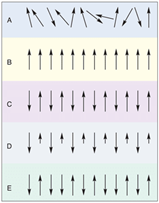
\includegraphics[width=0.9\columnwidth]{Gambar 1. Klasifikasi Magnetik.png}
    \caption{Classification of magnetic materials based on their response to external magnetic fields.}
    \label{fig:magnetic_classification}
\end{figure}

\begin{figure}[ht]
    \centering
    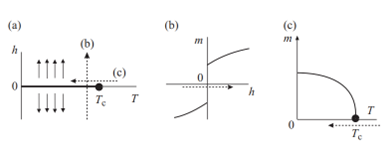
\includegraphics[width=0.9\columnwidth]{Gambar 4. Perubahan Fase Magnetik.png}
    \caption{Magnetic phase transitions showing the change in magnetization as a function of temperature.}
    \label{fig:magnetic_phase_transition}
\end{figure}

\begin{figure}[ht]
    \centering
    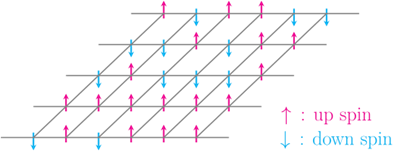
\includegraphics[width=0.9\columnwidth]{Gambar 5. Spin pada Model Ising.png}
    \caption{Spin orientations in the Ising model, showing the discrete nature of spin variables.}
    \label{fig:ising_model}
\end{figure}

\begin{figure}[ht]
    \centering
    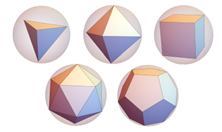
\includegraphics[width=0.9\columnwidth]{Gambar 6. The Platonic Solids.png}
    \caption{The Platonic solids representing the geometric basis for polyhedral spin models.}
    \label{fig:platonic_solids}
\end{figure}

\begin{figure}[ht]
    \centering
    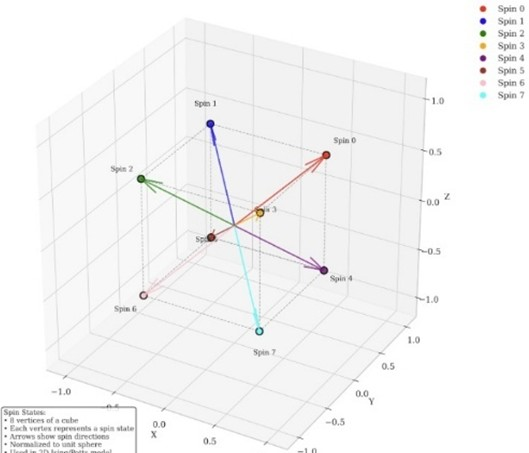
\includegraphics[width=0.9\columnwidth]{Gambar 7. Penommoran Titik Sudut pada Kubus.jpg}
    \caption{Vertex numbering on a cube, illustrating the eight possible spin orientations in the vertex-cubic model.}
    \label{fig:cube_vertices}
\end{figure}

\begin{figure}[ht]
    \centering
    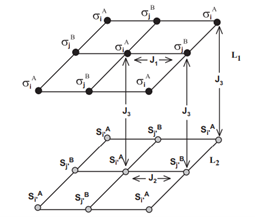
\includegraphics[width=0.9\columnwidth]{Gambar 8. Ilustrasi Kisi Persegi Berlapis.png}
    \caption{Illustration of layered square lattices, showing the structure used in the simulations.}
    \label{fig:layered_lattice}
\end{figure}

\begin{figure}[ht]
    \centering
    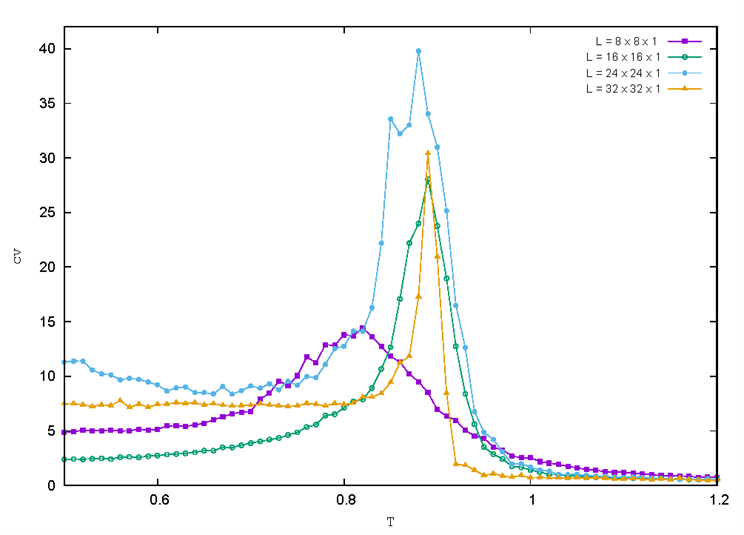
\includegraphics[width=0.9\columnwidth]{Gambar 9. Cv vs T pada Kisi Satu Lapis.png}
    \caption{Specific heat vs. temperature for a single-layer lattice, showing the peak that indicates a phase transition.}
    \label{fig:cv_single_layer}
\end{figure}

\begin{figure}[ht]
    \centering
    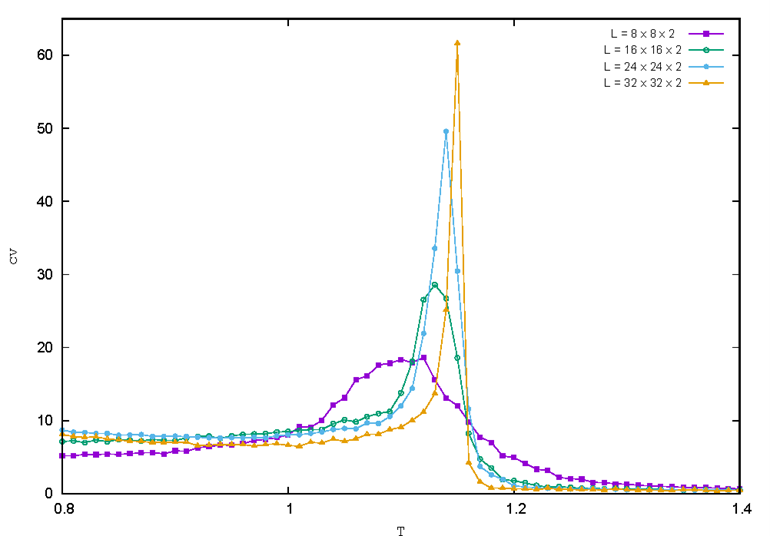
\includegraphics[width=0.9\columnwidth]{Gambar 10. Cv vs T pada Kisi 2 Lapis.png}
    \caption{Specific heat vs. temperature for a two-layer lattice, showing a sharper peak at a higher temperature.}
    \label{fig:cv_two_layer}
\end{figure}

\begin{figure}[ht]
    \centering
    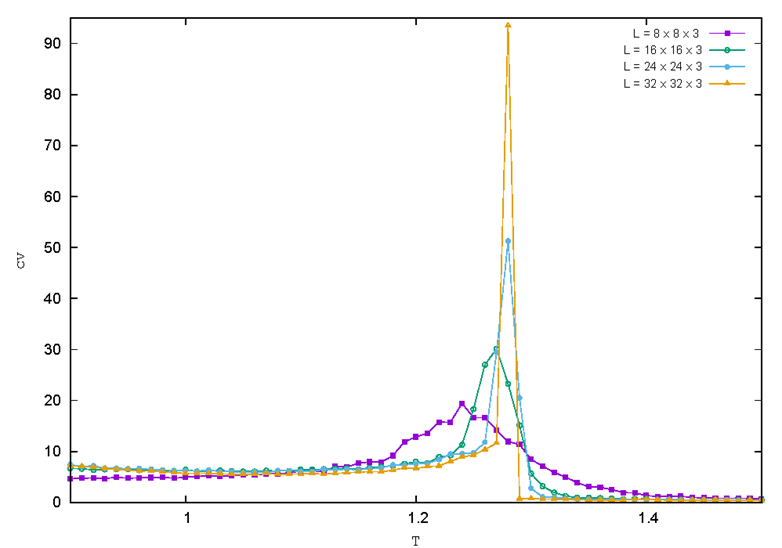
\includegraphics[width=0.9\columnwidth]{Gambar 11. Cv vs T pada Kisi 3 Lapis.png}
    \caption{Specific heat vs. temperature for a three-layer lattice, showing an even sharper peak at a higher temperature.}
    \label{fig:cv_three_layer}
\end{figure}

\begin{figure}[ht]
    \centering
    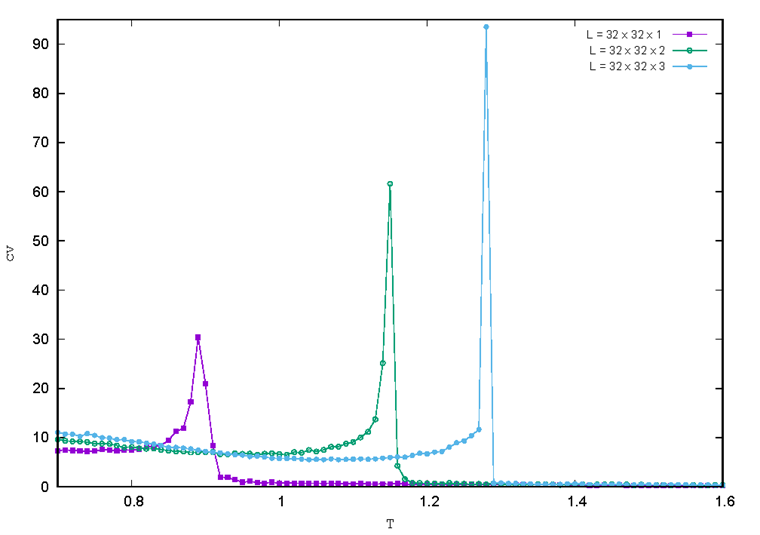
\includegraphics[width=0.9\columnwidth]{Gambar 21. Cv vs T pada Kisi 32 x 32.png}
    \caption{Specific heat vs. temperature for a 32×32 lattice, showing the effect of system size on phase transition characteristics.}
    \label{fig:cv_32x32}
\end{figure}

\begin{figure}[ht]
    \centering
    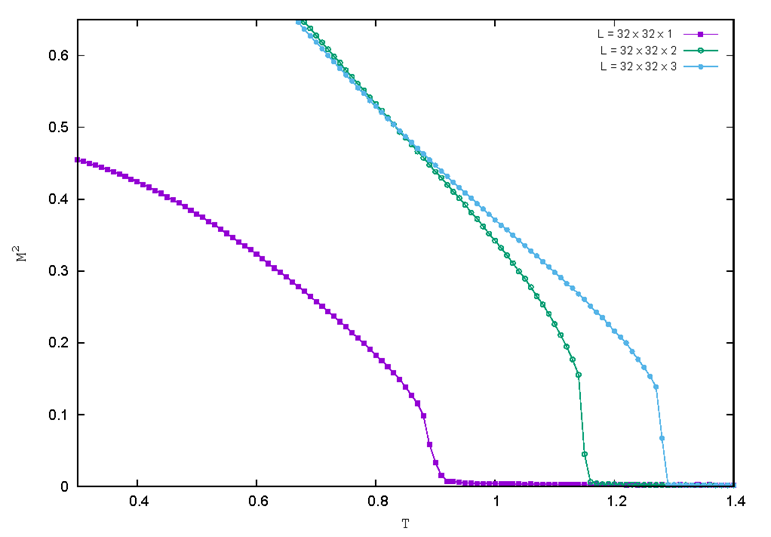
\includegraphics[width=0.9\columnwidth]{Gambar 25. M^2 vs T pada Kisi 32x32.png}
    \caption{Squared magnetization vs. temperature for a 32×32 lattice, showing the decay of magnetic order with increasing temperature.}
    \label{fig:m2_32x32}
\end{figure}

\begin{figure}[ht]
    \centering
    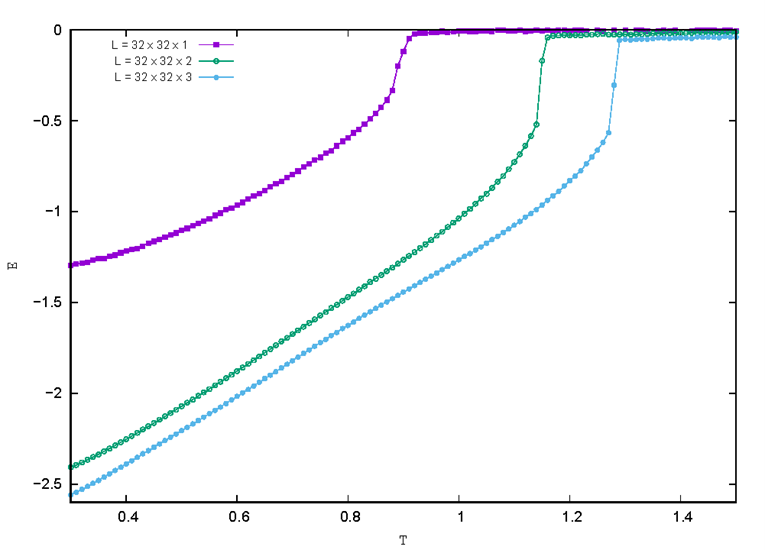
\includegraphics[width=0.9\columnwidth]{Gambar 29. E vs T pada Kisi 32x32.png}
    \caption{Energy vs. temperature for a 32×32 lattice, showing the increase in internal energy with temperature.}
    \label{fig:e_32x32}
\end{figure}

\end{document} 